\label{sec:whyworks}
Chapter~\ref{sec:method} built and validated \method{} \emph{operationally},
component by component: verified skeleton selection, reference duplication,
and the learned \gate{} together deliver strong rotation without losing
identity. None of that account so far explains \emph{why} those specific
components work, only that they do. This chapter closes that gap in two
steps: \emph{what} in the reference pathway actually carries identity into
the output (Sec.~\ref{sec:refverify}), and \emph{how much} of it survives as
the identity levers of Sec.~\ref{sec:identity}--\ref{sec:learned} are applied
(Sec.~\ref{sec:mechanism}). Both questions reduce to the same object---the
joint-attention budget Chapter~\ref{sec:method} introduced in
Sec.~\ref{sec:refgeometry} but did not yet analyze on its own terms.

\section{Why identity survives: verifying the reference-conditioning pathway}
\label{sec:refverify}
Sec.~\ref{sec:backbone} argued informally that a reference identity can survive
FLUX.2-klein's in-context conditioning without a dedicated ID-encoder branch,
provided (i) the VAE does not discard identity-relevant detail and (ii) the
transformer's joint attention actually reads that detail from the reference
block's \emph{content}, not merely its \emph{position} in the sequence. We
verify each link causally; full data and qualitative examples are in
App.~\ref{sec:appendix_causal}.

\paragraph{(i) The VAE preserves identity-discriminative detail.} We encode
then decode $34$ reference identities through the frozen VAE alone---no
denoising, no transformer---and compare each reconstruction
$I_{\mathrm{id}}^{\mathrm{recon}}$ to its original with AdaFace and PAEs
cosine (Table~\ref{tab:vaeroundtrip}). Reconstruction pairs score
$0.96$ AdaFace / $0.87$ PAEs against a same-set impostor baseline of
$0.01$/$0.04$---a $+0.96$/$+0.83$ separation. The lossy $8\times$-downsampling
codec is not the bottleneck: whatever the transformer does or does not do with
a reference, the identity evidence is still there to use.

\paragraph{(ii) Raw reference tokens do not yet look like a face embedding.}
Before attention runs, is identity already linearly readable from the
patch-embedded $C_{\mathrm{id}}$ tokens themselves, or does the transformer do
real work to extract it? We pool pre-RoPE, pre-attention $C_{\mathrm{id}}$
tokens (face-region, whole-image, background) for $35$ identities and test
their correspondence to the AdaFace embedding space by representational
similarity and top-1 nearest-neighbor agreement (Table~\ref{tab:tokengeometry}).
Every pooling---including the face region---is statistically indistinguishable
from a skeleton null control and from chance agreement. We report this
honestly as a null result: identity structure is \emph{not} already sitting in
the raw embedding; it is not extracted until the transformer's attention acts
on it.

\paragraph{(iii) The transformer causally reads reference content.} This
isolates the link that matters: does output identity track what is \emph{in}
the reference block, or could it be explained by the block merely occupying a
fixed slot in the sequence? Holding prompt, skeleton, seed, and the trained
\gate{} fixed, we vary only the pixels placed in the identity slot across four
conditions---the real photo of $A$, a swap to a different identity $B$, a
content-free grey block, and $A$ with the face region masked out---and score
every output against both $A$'s and $B$'s original photos
(Table~\ref{tab:causalswap_brief}, App.~\ref{sec:appendix_causal} Fig.~\ref{fig:causalswap}). Output identity
follows the swap: CSIM-to-$A$ is $0.34$ under the real photo and collapses to
$\leq\!0.02$ under every content ablation, while CSIM-to-$B$ rises to $0.28$
exactly when $B$'s photo---not $A$'s---occupies the slot. Masking only the
face region collapses identity as completely as a blank block, confirming the
effect is the \emph{face content} specifically, not merely a reference image
being present; the slot position is identical across all four conditions, so
position alone explains none of this.

\begin{table}[t]\centering\small
\setlength{\tabcolsep}{4pt}
\adjustbox{max width=\linewidth}{%
\begin{tabular}{lc c cc}
\toprule
Condition & $n$ & face det.\ & CSIM-to-$A$ & CSIM-to-$B$ \\
\midrule
normal-$A$ & $10$ & $8/10$ & $\mathbf{0.341}$ & $0.015$ \\
swap-$B$ & $10$ & $7/10$ & $-0.014$ & $\mathbf{0.280}$ \\
blank-ID & $10$ & $7/10$ & $-0.023$ & $-0.006$ \\
face-masked-$A$ & $10$ & $8/10$ & $-0.000$ & $-0.010$ \\
\bottomrule
\end{tabular}}
\caption[Content-vs-position causal swap]{\textbf{Content-vs-position causal swap} (mean AdaFace cosine over
detected faces; only the identity-slot pixels vary across conditions). Identity
follows reference \emph{content}, not slot position. Full table incl.\ the VAE
round-trip and token-geometry results: App.~\ref{sec:appendix_causal},
Table~\ref{tab:causalswap}.}
\label{tab:causalswap_brief}
\end{table}

\noindent Together: the VAE evidence survives (i), is not yet legible before
attention (ii), and the transformer causally reads it from content rather than
slot position (iii)---so \emph{attention to the identity block is the pathway
that turns reference content into output identity}, not an incidental
side-effect of where the block happens to sit. This is exactly why the
identity levers introduced earlier intervene on \emph{that pathway} rather
than on the reference pixels themselves: \dupid{} (Sec.~\ref{sec:identity})
adds physical key/value capacity to the identity block, and the learned
\gate{} (Sec.~\ref{sec:learned}) directly reweights its attention
logits---two different handles on the same softmax-normalized budget we
formalize next (Sec.~\ref{sec:mechanism}).

\section{One attention budget}
\label{sec:mechanism}
Sec.~\ref{sec:refverify} established \emph{what} the identity levers act
on---attention to the identity block's content; here we establish \emph{how
much} of it survives, and why every lever moves the same needle. The identity
levers of Sec.~\ref{sec:identity}--\ref{sec:learned} (duplication, id-first
ordering, the learned \gate{}) and the pose--identity
trade-off look unrelated; we show they are one mechanism. In the
joint attention, a generated query $q_i$ distributes a \emph{normalized} weight
over all key columns,
\begin{equation}
a_{ij}=\mathrm{softmax}_j\!\big(q_i^\top k_j/\sqrt{d}\big),\qquad \textstyle\sum_j a_{ij}=1 ,
\label{eq:attn}
\end{equation}
so the attention a face query can place on the identity block,
$s_{\mathrm{id}}=\sum_{j\in\mathrm{ID}} a_{ij}$, is one share of a fixed budget
that the structural control, text, and generated tokens also draw from. This
normalized-competition view---conditioning strength is a \emph{re-weighting} of
one budget, not an independent gain---is the principle behind in-context strength
controls such as OminiControl's $\log\gamma$ attention bias~\cite{ominicontrol},
ContextDrag's additive reference-key mask~\cite{contextdrag}, the image-prompt
scale of adapters~\cite{ipadapter}, and training-free attention
edits~\cite{masactrl,p2p}. We probe
$s_{\mathrm{id}}$ directly (recomputing softmax in a math attention backend so
the weights are available). Two findings (Fig.~\ref{fig:mechanism}A):
(i) adding the structural control \emph{reduces} $s_{\mathrm{id}}$---the source
of the pose--identity trade-off; (ii) each \dupid{} copy \emph{raises}
$s_{\mathrm{id}}$ monotonically---reference \emph{order} acts on the same
budget (App.~\ref{sec:appendix_ordering}).
Every effective lever is the same operation: re-allocate $s_{\mathrm{id}}$.

\paragraph{Causal verification (attention surgery).} Correlation is not enough.
We \emph{intervene}: holding everything else fixed, we add a bias $\log\gamma$ to
the identity columns' pre-softmax logits, which multiplies that block's
attention by $\gamma$~\cite{ominicontrol,contextdrag}---reproducing duplication's
\emph{effect} on the budget without copying any tokens. Sweeping $\gamma$ traces the \emph{same} rising
\csim{} curve as physically duplicating the block (Fig.~\ref{fig:mechanism}B):
scaling one block's attention by $\gamma{\approx}3$ recovers most of the
\dupid{} identity gain. This establishes \emph{causally} that \dupid's mechanism
is attention re-allocation; physical duplication only goes further because it
also adds token \emph{capacity}. The gate's own log-gain intervention
(Sec.~\ref{sec:learned}) is exactly this operation made learnable, per-step and
per-layer instead of a single hand-set constant.

\begin{figure}[t]\centering
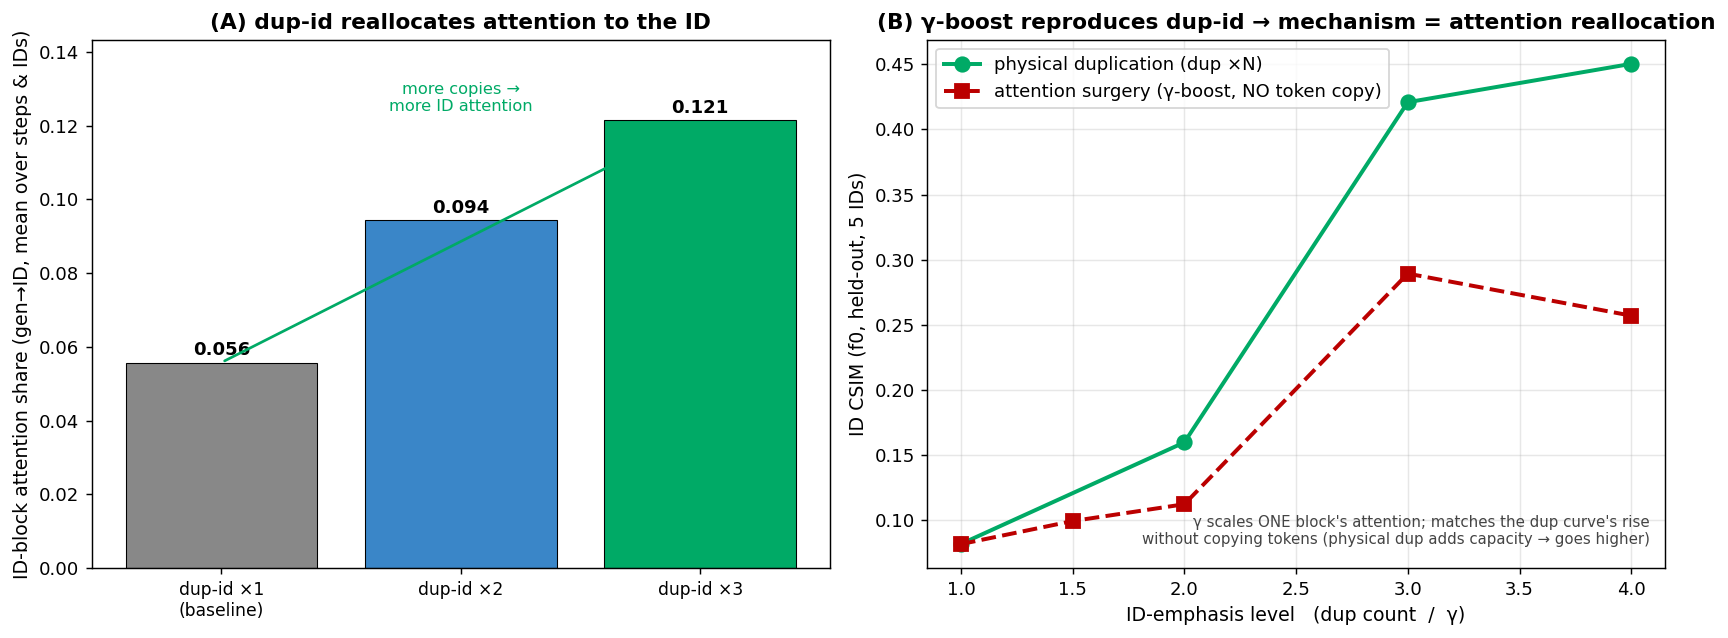
\includegraphics[width=\textwidth]{figures/mechanism.png}
\caption[One attention budget]{\textbf{One attention budget.} \textbf{(A)} The identity-block attention
share $s_{\mathrm{id}}=\sum_{j\in\mathrm{ID}}a_{ij}$: adding the structural control
\emph{lowers} it (the pose--identity trade-off), while each \dupid{} copy
\emph{raises} it monotonically---reference order has the same effect
(App.~\ref{sec:appendix_ordering}). Every lever is the same operation on $s_{\mathrm{id}}$.
\textbf{(B)} Attention surgery: biasing the identity columns' pre-softmax logits by
$\log\gamma$ traces the \emph{same} rising \csim{} curve as physically duplicating
the block, with $\gamma{\approx}3$ recovering most of the gain---causal evidence
that duplication acts by attention re-allocation.}
\label{fig:mechanism}
\end{figure}

\emph{When does it act?} Re-allocation is not a special case but the
\emph{default} at every query, attention layer, and denoise step (Eq.~\ref{eq:attn}). The
pose--identity trade-off \emph{triggers} the moment the structural block $S$ is
concatenated and competes for the same budget; symmetrically, each identity lever
takes effect precisely at the identity columns where that competition is
resolved. Because every lever is the \emph{same} localized operation, the fix
collapses to a single low-dimensional knob---exactly the one Sec.~\ref{sec:learned}
already made learnable.
